\documentclass[14pt, a2paper, portrait,innermargin=5mm,
blockverticalspace=5mm, colspace=5mm, subcolspace=3mm]{tikzposter}
% font size: The size of the text in the main body may be set as : 12pt, 14pt, 17pt, 20pt, or 25pt;
% paper size: Currently, paper sizes may be set to : a0paper, a1paper, or a2paper;
% orientation: Either landscape or portrait
\usepackage[utf8]{inputenc}
\usepackage[T1]{fontenc}

\usepackage{rustic}
\usepackage{lmodern}
\usepackage[sfdefault,lf]{carlito}
\usepackage{fontawesome}
\usepackage{blindtext}
\usepackage{comment}
\usepackage{hyperref}


\usepackage{listings}

\usetheme{Simple}
%\usetitlestyle{Empty}\usebackgroundstyle{Empty}

%--------------------------------------
%-------------- FARBEN

\usepackage[usenames, dvipsnames]{color} % um diese Color-Names zu verwenden: https://de.sharelatex.com/learn/Using_colours_in_LaTeX#!#Reference_guide z.B. \color{RubineRed}

\definecolor{GrafRed}{RGB}{102,0,34} %#660022
\definecolor{GrafBeige}{RGB}{226,212,186}

\definecolor{LightGrafRed}{RGB}{152,51,85} %#A3244E

%---------------- bei den Farben gibt es immer bg und fg, wobei bg Hintergrund und fg normalerweise Schriftfarbe ist. Dies ist zu definieren für backgroundcolor, framecolor, dann für titlefg/bgcolor, selbiges für (inner)blocktitle und blockbody, und ggf. für notefg/bgcolor
\colorlet{titlebgcolor}{GrafRed}
\colorlet{titlefgcolor}{GrafBeige}
\colorlet{blocktitlefgcolor}{GrafRed}

%---------------------- Code-Bsps
\definecolor{Text}{RGB}{0.36, 0.54, 0.66}
\definecolor{Element}{RGB}{0.53, 0.66, 0.42}
\definecolor{Attr}{RGB}{0.6, 0.4, 0.8}

\lstdefinelanguage{XML}
{
  morestring=[b]",
  morestring=[s]{>}{<},
  morecomment=[s]{<!--}{-->},
  morekeywords={xmlns,version,type,canonicalRef,metr,real,target}% list your attributes here
}

\lstset{language=XML,
showspaces=false,
showtabs=false,
basicstyle=\ttfamily,
columns=fullflexible,
breaklines=true,
showstringspaces=false,
breakatwhitespace=true,
escapeinside={(*@}{@*)},
basicstyle=\ttfamily\footnotesize,
stringstyle=\color{Text},
commentstyle=\color{Element}\upshape,
keywordstyle=\color{SpringGreen}\bfseries,
}


%---------------------------- Title-Infos und Package-Wirrwarr

\title{{\rustfamily\bfseries Graz Repository of Ancient Fables}}
%\author{Prof. Dr. Ursula Gärtner, Sarah Lang}
%\date{\today}
\author{Institute for Classics \& ZIM-ACDH, KFU Graz}
%\institute{Institute of Classics, Karl-Franzens-Universität Graz}
\titlegraphic{\hspace{2cm}
\includegraphics[height=7.5cm, right]{graf-logo-beige.png}}

%----------------------------------------------------------------------
% Title definieren
\definetitlestyle{sampletitle}{
width=\paperwidth, linewidth=2pt, innersep=5pt,
titletotopverticalspace=0mm, titletoblockverticalspace=10mm
}{
\begin{scope}[line width=\titlelinewidth]
\draw[color=blocktitlebgcolor, fill=titlebgcolor]
(\titleposleft,\titleposbottom) rectangle (\titleposright,\titlepostop);
\end{scope}
}
%---------------------- und so weiter... geht alles nicht..
\settitle{\begin{tabular*}{0.8\textwidth}{r p{0.7\textwidth}}%
\@titlegraphic & \vbox{%
\centering%
\color{titlefgcolor} {\bfseries \Huge \sc \@title \par}
\vspace*{1em}
{\huge \@author \par} \vspace*{0.5em} {\LARGE \@institute}
} \end{tabular*}
}

\usetitlestyle{sampletitle}


%line-overflow meiden, dazu hinter begin{doc} \sloppy
\setlength{\emergencystretch}{2pt}

 %--------------------- PDF-Info
 \hypersetup{
    pdftitle={GRaF},
    pdfauthor={Sarah Lang},
    pdfsubject={GRaF project},
    pdfkeywords={GRaF; GAMS repository; ancient fables},
    colorlinks=false,           % no link border color
    pdfa,
}


 
 %--------------------------------------
 % new commands für CV-Icons
 
 % 1. Argument=favicon; 2. Argument=Text; 3.+4.=ColorName; 5.Schriftgröße z.B. \Large
 
 % cvicon command
 \newcommand{\cvicon}[4]{%
\vspace{0.5pt}\begin{minipage}[t]{0.12\textwidth}\vspace{0pt}%
 \begin{tabular*}{0.125\textwidth}{c c}%
{\color{#3}\centering\Large #1} & \phantom{}\\%  
{\color{#4}\footnotesize\sffamily \parbox[t]{\textwidth}{\centering#2}} & \phantom{}\\%
\end{tabular*} \end{minipage} \hfill%
  }
 
  % bigicon command
 \newcommand{\bigicon}[4]{%
\vspace{0.5pt}\begin{minipage}[t]{0.12\textwidth}\vspace{0pt}%
 \begin{tabular*}{0.125\textwidth}{c c}%
{\color{#3}\centering\Huge #1} & \phantom{}\\%  
{\color{#4}\Large\sffamily \parbox[t]{\textwidth}{\centering#2}} & \phantom{}\\%
\end{tabular*} \end{minipage} \hfill%
  }

  % bullettpoint command
 \newcommand{\bullettpoint}[5]{%
\vspace{0.35em}\begin{minipage}[t]{\textwidth}\vspace{0pt}%
 \begin{tabular*}{0.125\textwidth}{c c}%
{\color{#3}\centering#5 #1\phantom{}} & {\color{#4}#5\sffamily \parbox[t]{\textwidth}{#2}}\\%  
\end{tabular*}\vspace{0.15em} \end{minipage}\hfill%
  }
%----------------------------------------------------------------




\begin{document}

\maketitle

\block{{\rustfamily The Project: Fabula docet -- Who wants sour grapes}?}
{
\begin{minipage}[t]{0.35\textwidth}\vspace{0pt}

\subsection*{\Large The Project}
Fables are short, easy to translate \&  thus constitute a great medium for introducing pupils to literary studies in Latin and Ancient Greek class. They have, however, mostly been frowned upon by science as ``children’s stories''. 
\bigskip

The goal of the project is to innovatively explore the concept of the \textbf{``digital school book''}, created by the pupils themselves but grounded in up-to-date scientific research on fables; \textbf{not} mainly to provide \textbf{an interactive learning platform}. 

\subsection*{\Large Technical Aspects}
Apart from providing the original \textbf{fable texts in TEI} annotated form -- scientific comments as well as simple vocabulary help--, the repository (available via the FEDORA based asset management system GAMS) is completed with didactic materials as well as scientific introductions. 
\bigskip

It thereby challenges the Digital Humanities to explore this \textbf{new kind of medium} - somewhere between a \textbf{digital (scholarly) edition} and a \textbf{learning platform}. The \textbf{digital edition (``fable repository'')} is the centrepiece of the project and contains a \textbf{selection of fables} (Phaedrus, Avian, Babrius, Aesop), providing enrichment of the original texts with vocabulary help, translations, explanations and parallel texts. 


\end{minipage}\hfill\hspace{1em}
\begin{minipage}[t]{0.28\textwidth}\vspace{0pt}

\coloredbox[width=0.95\textwidth,bgcolor=GrafBeige,fgcolor=GrafRed,framecolor=GrafBeige]{TEI example (non-final)


\lstinputlisting{graf.xml}

\bigskip


Examples of the repository (beta, test server): \small\protect\url{censored_no-link-or-QR-available} \normalsize
\begin{tikzfigure}
            
\includegraphics[width=0.2\textwidth]{graf-logo-schwarz.png}\hspace{1em}
            
\includegraphics[width=0.2\textwidth]{graf-logo-schwarz.png}
        \end{tikzfigure}
}


\end{minipage}\hfill\hspace{0.5em}
\begin{minipage}[t]{0.26\textwidth}\vspace{0pt}
\begin{tikzfigure}
            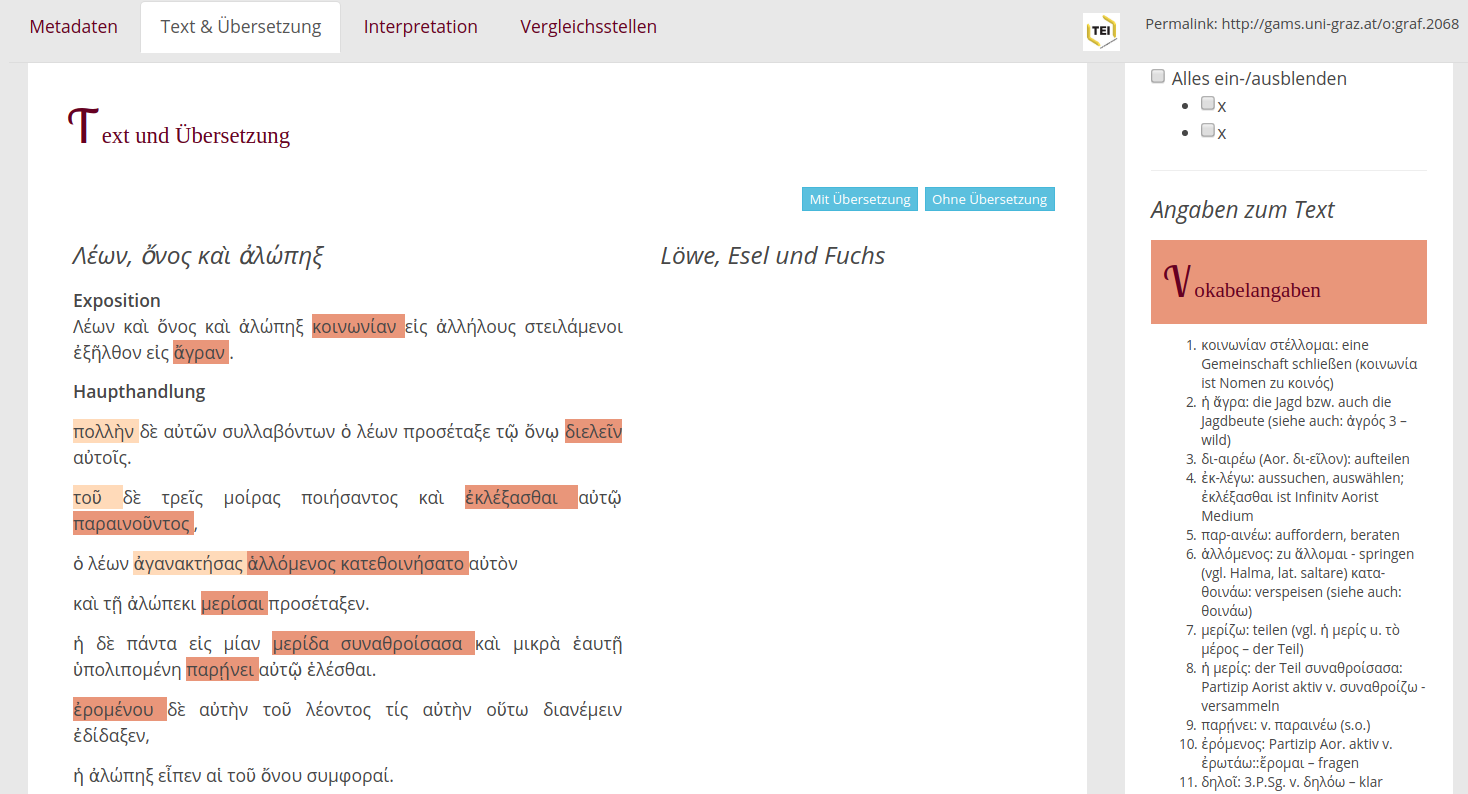
\includegraphics[width=0.95\textwidth]{text.png}
        \end{tikzfigure}
        \begin{tikzfigure}
            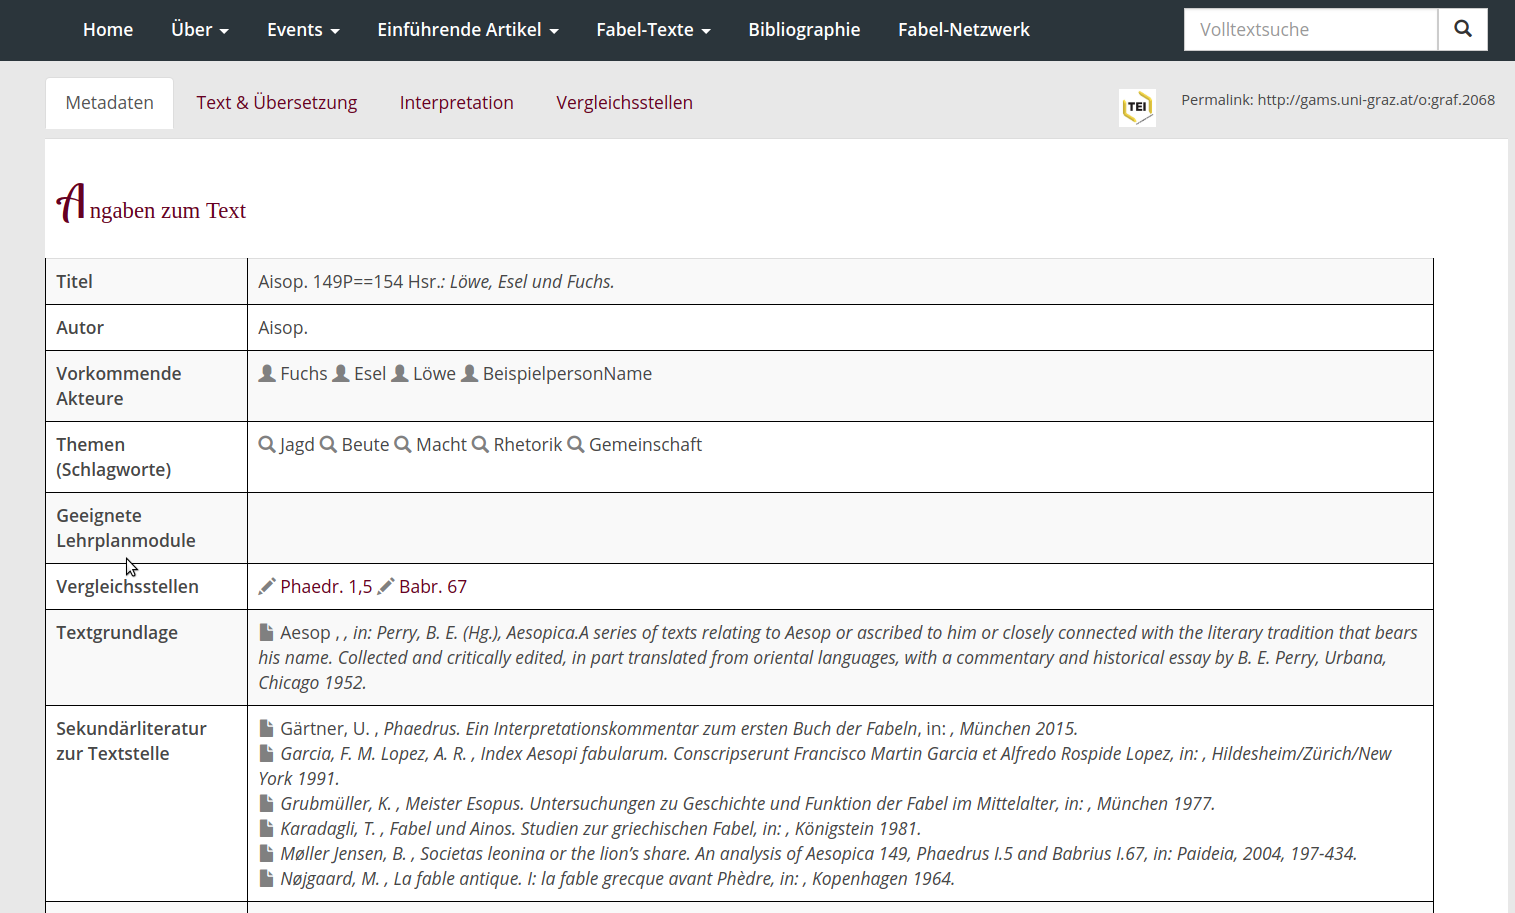
\includegraphics[width=0.95\textwidth]{angaben.png}
        \end{tikzfigure}
        \begin{tikzfigure}
            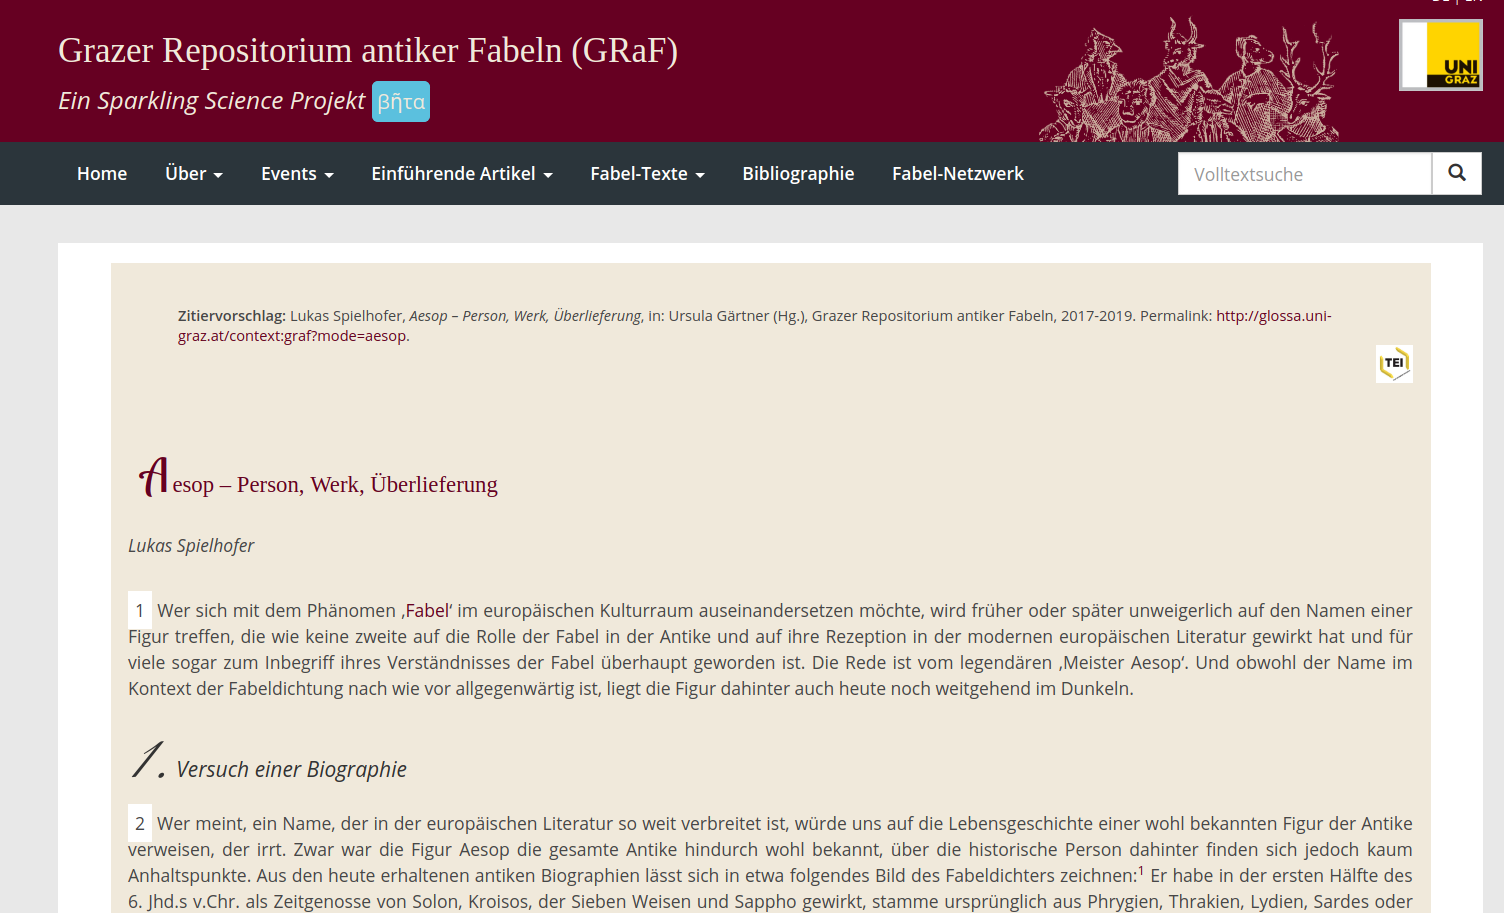
\includegraphics[width=0.95\textwidth]{intro.png}
        \end{tikzfigure}

\end{minipage}\hfill

\vspace{1.5em}

\bigskip

%------------ das hier ginge auch mit dem nicht TikzPoster-eigenen \colorbox{GrafRed}{Inhalt}, schaut aber nicht ganz so schön aus und passt sich nicht von allein an die Poster-Box an..

\coloredbox[roundedcorners,bgcolor=GrafRed,fgcolor=GrafBeige,framecolor=GrafRed]{
      \Huge\begin{minipage}[c]{0.95\textwidth} % Start the right-hand side of the page
      \bigskip
\bigicon{\faUsers}{Schools}{GrafBeige}{GrafBeige}
\bigicon{\faLaptop}{Repository}{GrafBeige}{GrafBeige}
\bigicon{\faUniversity}{Citizen Science}{GrafBeige}{GrafBeige}
\bigicon{\faKeyboardO}{{\large Digital Humanities}}{GrafBeige}{GrafBeige}
\bigicon{\faGraduationCap}{University}{GrafBeige}{GrafBeige} \phantom{  }

\end{minipage}
}

\bigskip
%\vspace{1em}

%\begin{minipage}[t]{0.45\textwidth}\vspace{0pt}
%\faClockO\phantom{ } 2017--2019
%\phantom{ }\faLaptop\phantom{ } Beta version of the repository on the test server \\
%\phantom{ }\faCheck\phantom{ } first `run' in schools completed
%\phantom{ }\faArrowCircleRight\phantom{ } \textbf{now}: integration of the first `real', non-test data
%\end{minipage}\hfill\hspace{1em}
%\begin{minipage}[t]{0.41\textwidth}\vspace{0pt}
%\faUniversity\phantom{ } `Grazer Latein-Tage' (once per year)
%\phantom{ }\faUsers\phantom{ } pupil's conference
%\phantom{ }\faGraduationCap\phantom{ } workshops
%\phantom{ }\faGraduationCap\phantom{ } scientific introductions as part of the repository \\
%\phantom{ }\faAt\phantom{ } creation of a `fable network' for scientists
%\normalsize
%\end{minipage}\hfill
}


\begin{columns}
   \column{0.36}
    \block{}{
    \coloredbox[width=0.3\textwidth,roundedcorners,bgcolor=GrafBeige,fgcolor=GrafBeige,framecolor=GrafBeige]{
        \begin{tikzfigure}
            
\includegraphics[width=0.07\textwidth]{zim_rot.png}
            
\includegraphics[width=0.07\textwidth]{kfFarbe.jpg}\hspace{0.5em}
            
\includegraphics[width=0.07\textwidth]{graf-logo-rot.png}
            
            \vspace{1em}
            \bigskip


\includegraphics[width=0.07\textwidth]{oead-transp.png}\hspace{0.5em}

\includegraphics[width=0.07\textwidth]{bmbwf.png}\hspace{0.5em}

\includegraphics[width=0.07\textwidth]{gamslogo.png}

\vspace{1em}
            \bigskip
            
\includegraphics[width=0.23\textwidth]{sparklingScience.jpg}
            
            \bigskip\phantom{}
        \end{tikzfigure}
         }
    }
    
    \column{0.27}
    \block{{Contact}}{
      \begin{minipage}[t]{0.25\textwidth}\vspace{0pt}
      \bullettpoint{\faUser}{ Univ.-Prof. Dr.phil. Ursula Gärtner}{}{}{}\\
\bullettpoint{\faUniversity}{Institut für Klassische Philologie}{}{}{}
\bullettpoint{\faMapMarker\phantom{}}{Universitätsplatz 3/II, 8010 Graz}{}{}{}
\bullettpoint{\faPhone}{Tel: +43 (0)316 380 -- 2430}{}{}{}
\bullettpoint{\faAt}{\protect\url{klassphil@uni-graz.at}}{}{}{}
 \end{minipage}\hfill
       \bigskip
      
      \coloredbox[width=0.24\textwidth,roundedcorners,bgcolor=GrafRed,fgcolor=GrafBeige,framecolor=GrafRed]{
       \begin{minipage}[t]{0.25\textwidth}\vspace{0pt}
     \bullettpoint{\faCode}{\protect\url{sarah.lang@uni-graz.at}}{GrafBeige}{GrafBeige}{\large}\\
\bullettpoint{\faLaptop}{Beta version of the repository on the test server}{GrafBeige}{GrafBeige}{\small}\\
\bullettpoint{\faCheck}{first `run' in schools completed}{GrafBeige}{GrafBeige}{\small}\\
\bullettpoint{\faArrowCircleRight}{\textbf{now}: integration of the first `real', non-test data}{GrafBeige}{GrafBeige}{\small}
 \end{minipage}\hfill
       }       


   
    }
    \column{0.32}
    \block{}
    {
    \coloredbox[width=0.29\textwidth,roundedcorners,bgcolor=GrafRed,fgcolor=GrafRed,framecolor=GrafRed]{
    \begin{tikzfigure}
            \includegraphics[width=0.23\textwidth]{fabelbuch.jpg}
        \end{tikzfigure}
        \phantom{ }
       } 
       
       \bigskip
      
      \coloredbox[width=0.29\textwidth,roundedcorners,bgcolor=GrafBeige,fgcolor=GrafRed,framecolor=GrafBeige]{
     \bullettpoint{\faMousePointer}{\url{https://gams.uni-graz.at/graf}}{}{}{}\\
\bullettpoint{\faClockO}{\textbf{Project duration:} 01.10.2017--30.09.2019}{}{}{}\\
       } 
      
    }
    
\end{columns}

\end{document}
